%!TEX TS-program = xelatex
%!TEX encoding = UTF-8 Unicode

\documentclass[12pt]{article}
\usepackage{geometry}                % See geometry.pdf to learn the layout options. There are lots.
\geometry{a4paper,top=2cm}
\usepackage[parfill]{parskip}    % Activate to begin paragraphs with an empty line rather than an indent
\usepackage{graphicx}
\usepackage{amsmath}
\usepackage{amssymb}
\usepackage{mathtools}
\usepackage{physics}
\newcommand{\be}{\begin{equation}}
\newcommand{\ee}{\end{equation}}
\usepackage[thicklines]{cancel}
\usepackage[colorlinks=true,citecolor=blue,linkcolor=blue,urlcolor=blue]{hyperref}
\usepackage{booktabs}
\usepackage{csquotes}
\usepackage{qcircuit}
\usepackage{circledsteps}
\usepackage{nicefrac}
\usepackage{fontspec,xltxtra,xunicode}
\usepackage{xcolor}
\usepackage{simplewick}
\defaultfontfeatures{Mapping=tex-text}

\newcommand{\polv}{\ensuremath{\updownarrow}}
\newcommand{\polh}{\ensuremath{\leftrightarrow}}
\newcommand{\poldr}{\rotatebox[origin=c]{45}{\ensuremath{\leftrightarrow}}}
\newcommand{\poldl}{\rotatebox[origin=c]{-45}{\ensuremath{\leftrightarrow}}}
\newcommand{\bigzero}{\mbox{\normalfont\Large\bfseries 0}}
\newcommand{\vecrp}{\ensuremath{\vec{r}^{\,\prime}}}
\newcommand{\vecnr}{\ensuremath{\vec{\nabla}_{\!r}}}

\title{Advanced Quantum Mechanics\\Class 01}
%\author{The Author}
\date{March 14, 2023}                                           % Activate to display a given date or no date

\begin{document}
\maketitle

%\setcounter{section}{2}

%%% 1 OK

\section{Postulates of Quantum Physics}

Here: generalization of previous results for
the photon polarization and spin 1/2
-- give the general conceptual framework
but does not provide the tools for
solving specific problems.
This requires modeling (simplifications, approximations),
heuristic arguments $\Leftarrow$ \emph{not} derivable within
the general framework.

The discussion will be divided into three parts
\begin{enumerate}
\item State vectors and physical properties
\item Time evolution
\item Approximations and modeling (short discussion)
\end{enumerate}

\subsection{State vectors and physical properties}
\begin{quote}
\emph{The superposition principle}
\end{quote}

\emph{Postulate I:} the space of states.

$\ket{\varphi}$: state vector, element of a complex Hilbert
%%% 02 OKAY
 space $H$ (space of states).
 $\ket{\varphi}$ defines completely the properties of a quantum system.
Convenience: choose $\|\varphi\|^2 = \bra{\varphi}\ket{\varphi} = 1$.
In general, description in terms of vectors in a $H$
implies the superposition principle (linearity):
-- $\ket{\varphi}$, $\ket{\chi}$ in $H$ the vector $\ket{\psi}$
\be
\ket{\psi} = \frac{\lambda\ket{\varphi}+\mu\ket{\chi}}{\|\lambda\ket{\varphi}+\mu\ket{\chi}\|^2}
\ee
for $\lambda$ and $\mu$ complex number, is also in $H$
and represents a physical state.

\emph{Postulate II:} probability amplitudes and probabilities.

$\ket{\varphi}$ represents a state,
$\ket{\chi}$ represents another state $\Rightarrow$
there exists a \emph{probability amplitude}
\be
a(\varphi \to \chi) = \bra{\chi}\ket{\varphi}
\ee
of finding the state $\ket{\varphi}$ in $\ket{\chi}$. Here,
$\bra{\varphi}\ket{\chi}$ is the scalar product in $H$.
The \emph{probability} for $\ket{\varphi}$ to pass the test $\ket{\chi}$ is given by (the Born rule):
%%% 03 OKAY
\setcounter{equation}{1}
\be
P(\varphi \to \chi) = |a(\varphi \to \chi)|^2 = |\bra{\chi}\ket{\varphi}|^2
\label{eq:g2}
\ee
\emph{Remarks:}
\begin{itemize}
\item as a rule, assume vectors normalized to unity.
When not the case, Eq.~\eqref{eq:g2} above becomes:
\be
P(\varphi \to \chi) = \frac{|\bra{\chi}\ket{\varphi}|^2}{\|\varphi\|^2\|\chi\|^2}
\ee
%
\item $\ket{\varphi}$ and $\ket{\varphi^\prime} = e^{i\beta}\ket{\varphi}$ represent the \emph{same
physical state}: physical state is represented by
a vector up to a phase ($\ket{\varphi}$ and $\ket{\varphi^\prime}$ are \emph{a ray}).
But relative phases matter:
\be
\lambda\ket{\varphi}+\mu\ket{\chi}
\text{ different state from }
\lambda\ket{\varphi^\prime}+\mu\ket{\chi}
\ee
%
\item here, \emph{pure states} only $\to$ maximal information
about the physical state.
Mixed states, when information is incomplete
on the physical states, will be dealt with
further ahead [state (density) operator]
%
\item quantum \emph{system} $\times$ quantum \emph{particle}: for many
particles, it is often impossible to attribute a
%%% 04 OKAY
state vector to an individual particle, only to
the whole
\end{itemize}

\emph{Postulate III:} physical properties and operators.

Physical property $\mathcal{A}$: spin component in direction $\hat{n}$, energy, momentum, angular momentum, etc.
$\Rightarrow$ With every $\mathcal{A}$, one associates an operator $\hat{A}$ in $H$ which acts on vectors of $H$.
Suppose an $\mathcal{A}$ represented by a $\hat{A} = \hat{A}^\dagger$:
\be
\hat{A}\ket{n} = a_n \ket{n}
\ee
(we assume the $a_n$ are nondegenerate, for now)
Then one can write the spectral representation of $\hat{A}$
\be
\hat{A} = \sum_n \ket{n} a_n \bra{n} = \sum_n \op{n}
\ee
\begin{itemize}
\item if the system is in state $\ket{\varphi} = \ket{n}$:
\[
\hat{A}\ket{\varphi} = \sum_{n^\prime} a_{n^\prime}\ket{n^\prime}\bra{n^\prime}\ket{n} = a_n\ket{n}
\]
so $\mathcal{A}$ takes the exact numerical value $a_n$.
%
\item if $\ket{\varphi} \neq \ket{n}$, postulate II:
\be
P_n(\ket{\varphi}\to a_n) = |\bra{n}\ket{\varphi}|^2
\ee
where $P_n$ is the probability of measuring $a_n$.
\end{itemize}
%%% 05 OKAY
Average value (expectation value) of $\mathcal{A}$ is given by
\be
\begin{aligned}
\ev{A}_\varphi
&=\sum_n P_n a_n = \sum_n |\bra{n}\ket{\varphi}|^2 a_n\\
&=\sum_n \bra{n}\ket{\varphi}^* \bra{n}\ket{\varphi} a_n = \sum_n \bra{\varphi}\ket{n} \bra{n}\ket{\varphi} a_n \\
&= \bra{\varphi} \overbrace{\sum_n a_n \op{n}}^{\hat{A}} \ket{\varphi}
=\bra{\varphi}\hat{A}\ket{\varphi}
\end{aligned}
\ee
Experimentally, to determine if $\ket{\varphi}$ is in $\ket{n}$,
$n = 1,2,\ldots,N$:

\begin{minipage}{0.5\textwidth}
\begin{enumerate}
\item imagine a ``generalized Stern-Gerlach'' (GSG) experiment, with $N$ exit channels.
\item carry out a series of $\mathcal{N}$ tests on systems
all being in $\ket{\varphi}$, \textit{i.e.} all \emph{prepared in the
state} $\ket{\varphi}$.
\end{enumerate}
\end{minipage}%
\quad%
\begin{minipage}{0.5\textwidth}
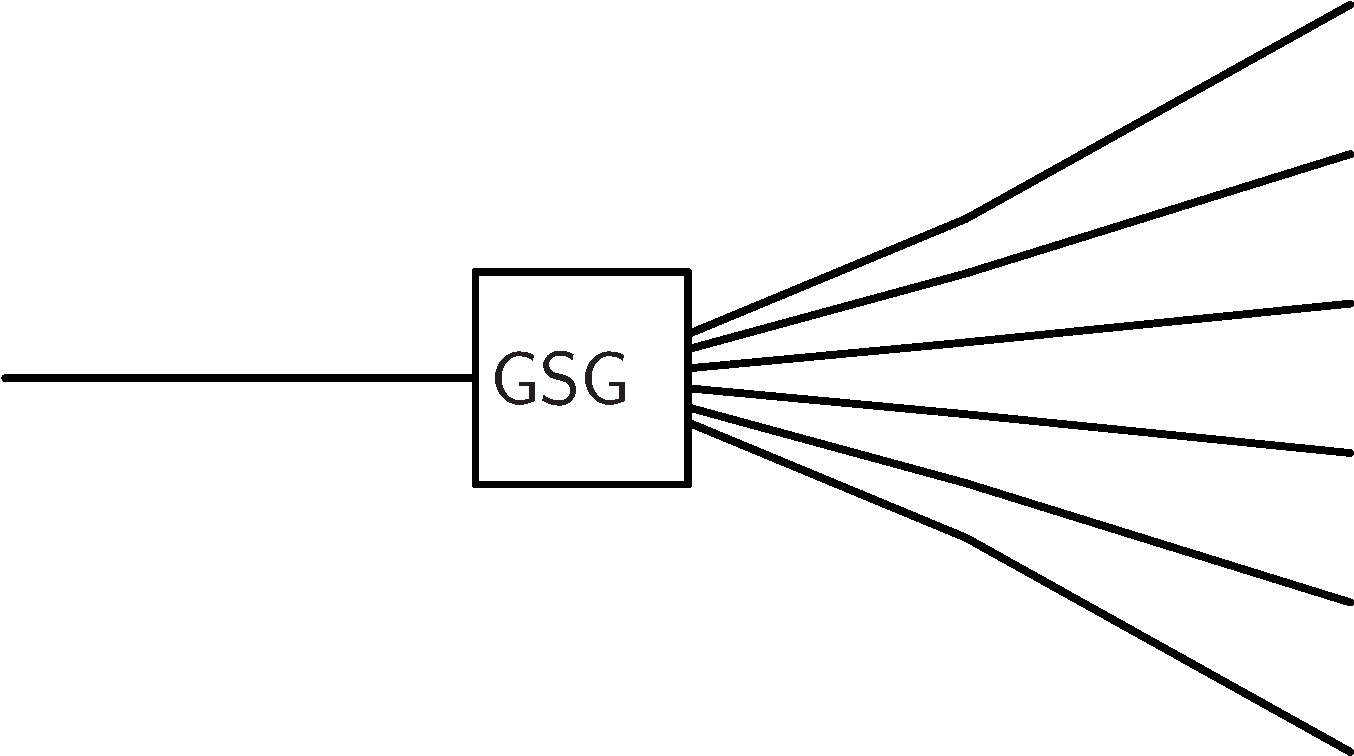
\includegraphics[width=0.8\textwidth]{Figures/GeneralizedSternGerlach.pdf}~
\raisebox{1.5cm}{$\left.\rule{0pt}{2cm}\right\}\,{N}$}
\end{minipage}

For $\mathcal{N}$ sufficiently large, the
average of $\mathcal{A}$ in $\ket{\varphi}$, $\ev{A}_\varphi$, is
\be
\ev{A}_\varphi = \lim_{\mathcal{N}\to\infty} \frac{1}{\mathcal{N}} \sum_{p=1}^{\mathcal{N}} \mathcal{A}_p
\ee
where $\mathcal{A}_p$ is the result of the $p$-th measurement (one click).
$\mathcal{A}_p$ varies, in general, from one test to another,
but in each test, $\mathcal{A}_p$ is one of the $a_n$.
%%% 06 OKAY
In case $a_n$ is degenerate:
\be
\ket{\varphi} = \sum_{n,r}\ket{n_r}\underbrace{\bra{n_r}\ket{\varphi}}_{C_{nr}} = \sum_{n,r} C_{nr}\ket{n,r}
\ee
The probability of observing $a_n$:
\be
\begin{aligned}
p(a_n)
&= \sum_r |C_{nr}|^2 = \sum_r \bra{n,r}\ket{\varphi}^* \bra{n,r}\ket{\varphi}\\
&= \sum_r \bra{\varphi}\ket{n,r}\bra{n,r}\ket{\varphi}
= \bra{\varphi}\underbrace{\sum_r\op{n,r}}_{\hat{P}_n}\ket{\varphi}\\
&=\bra{\varphi}\hat{P}_n\ket{\varphi}
\end{aligned}
\ee
As in the nondegenerate case, a large number
of measurements carried out in identically-prepared
systems leads to the average value of $\mathcal{A}$:
\be
\begin{aligned}
\ev{\hat{A}}_\varphi
&= \sum_n a_n p(a_n) = \bra{\varphi}
\underbrace{\left(
\sum_{n,r}\ket{n,r}a_n\bra{n,r}
\right)}_{\hat{A}}%
\ket{\varphi}\\
&= \bra{\varphi}\hat{A}\ket{\varphi}
\end{aligned}
\ee

Simplest Hermitian operator: projector on a vector in $H$
subjecting a system to a $\ket{\chi}$ \emph{test}
is equivalent to a \emph{measurement} of
\be
\hat{P}_\chi = \op{\chi}
\ee
%%% 07 OKAY
-- result is \emph{1} if the system passes the test $\ket{\chi}$, and \emph{0} if it does not
$\Rightarrow$ \emph{testing} and \emph{measuring} closely related.
\begin{itemize}
\item\emph{Measurement:} when interested in the eigenvalues of an $\hat{A}$.
\item\emph{Test:}        when interested in the probability of finding an eigenvalue of $\hat{A}$.
\end{itemize}

One must differentiate between two kinds of
measurements: destructive (atoms / photons absorbed on a screen) and nondestructive (ideal; laser excitation,
deexcitation in a cavity -- see Fig.~4.1 of Le~Bellac).

In general, a quantum system, prepared in a
$\ket{\varphi}$ state, that passes a $\ket{\chi}$ test will be
found in the state $\ket{\chi}$ \emph{immediately} after the test:
\be
\ket{\varphi} \xrightarrow[\ket{\chi}]{\text{test of}}\frac{\hat{P}_\chi\ket{\varphi}}{\|\hat{P}_\chi\ket{\varphi}\|}
\ee
%%% 08 OKAY
The system has undergone an irreversible
transition from $\ket{\varphi}$ to $\ket{\chi}$: wave function has ``collapsed''.

\emph{WFC postulate} -- complement to Postulate II.

If a system is initially in a state $\ket{\varphi}$,
and if the result of an ideal measurement
of a physical property $\mathcal{A}$ is $a_n$, then
immediately after this measurement the
system is in the state projected on the
subspace of the eigenvalue $a_n$:
\be
\ket{\varphi} \to \ket{\psi} = \frac{\hat{P}_n\ket{\varphi}}{(\bra{\varphi}\hat{P}_n\ket{\varphi})^{\nicefrac{1}{2}}}
\ee
where this postulate is relevant for nondestructive measurements.
If $a_n$ degenerate $\to$ need to measure
simultaneously another physical
quantity $\mathcal{B}$ compatible with
$\mathcal{A}$: $[\hat{A},\hat{B}] = 0$.
The $a$ and $b$ eigenvalues of $\hat{A}$ and $\hat{B}$ specify the state completely $\to$ if not, find still another, $\mathcal{C}$.

%%% 09 OKAY

All this is radically different from the measurement
process in classical physics, where we measure a pre-existing property.
In quantum physics, the measurement of
a $S_x$ component of a spin-1/2 system
in the state $\ket{+}$ \emph{does not reveal} a value
of $S_x$ existing before the measurement;
since we find a ``spread'' between $\ket{+}$ and $\ket{-}$,
$S_x$ \emph{does not exist} before it is measured.

\end{document}
